\documentclass[12pt,twoside]{article}
\usepackage{lscape,graphicx,setspace,multicol,sidecap,fullpage}
\renewcommand{\thesection}{\arabic{section}}
\title{Quantitative geomorphology of the White Mountains
(California), using detrital Apatite Fission Track thermochronology}
\author{Pieter Vermeesch\\
Institute of Isotope Geology and Mineral Resources, ETH-Z\"{u}rich
\\ pieter.vermeesch@erdw.ethz.ch}
\begin{document}
\maketitle
\section*{Abstract}

Detrital thermochronology has been  proposed as a method for measuring
average basin-wide  erosion rates. This  paper illustrates how  to use
detrital apatite fission track (AFT) thermochronology to map out where
in a basin erosion takes place. Five samples of detrital AFT ages were
collected on an alluvial fan that  is fed by the Marble Creek drainage
basin in  the northern White Mountains (California).   Using a digital
elevation  model  to  characterize  the  basin hypsometry  and  a  few
published basement samples to constrain the age-elevation curve of the
catchment, the detrital AFT distribution was predicted.  Comparing the
observed with  the predicted age distributions  reveals that localized
rock fall events  provide the sediment source of  the currently active
Marble  Creek, but  a composite  sample from  the entire  alluvial fan
indicates   that  over   longer  timescales,   the   entire  catchment
contributes  material  to the  debris-flow  dominated  fan, with  more
material being derived  from lower elevations than from  higher up the
Marble Creek  Canyon.  The observed  AFT age distribution  is compared
with   the  hypsometric   predictions  using   the   ``Cumulative  Age
Distribution''  (CAD)  which is  the  cumulative  distribution of  the
measured  ages. In  contrast with  probability density  estimators and
their cumulative equivalents, the  CAD requires no numerical smoothing
while properly accounting for (unequal) measurement uncertainties.

\section{Introduction}
\label{sec:introduction}

Radiometric   cooling   ages   ($^{40}$Ar/$^{39}$Ar,  fission   track,
(U-Th)/He) of exhumed fault  blocks generally increase with elevation. 
For  catchments draining  such  terranes, it  is  possible to  predict
detrital  age  distributions  if  the  relationship  between  age  and
elevation is either  assumed or known, if the  catchment hypsometry is
known,  and under  some  additional assumptions,  which are  discussed
below.\\

A few studies  have explored this for the  $^{40}$Ar/$^{39}$Ar system. 
If  erosion   is  in   a  steady  state   over  geologic   time,  then
$^{40}$Ar/$^{39}$Ar  cooling ages  are expected  to  decrease linearly
with  depth, or increase  linearly with  elevation.  In  a theoretical
study,  {\it  Stock  and  Montgomery}  [1996] argue  that,  under  the
assumption of a thermal gradient,  the {\it range} of detrital cooling
ages can be used to  estimate (paleo-)relief.  Going one step further,
{\it  Brewer et  al.}  (2003)  proposed a  method to  estimate average
basin-wide erosion rates  by matching the {\it shape}  of detrital age
distributions with the area-elevation  curve (= ``hypsometry'') of the
catchment.  In a recent paper, {\it Ruhl and Hodges} [2005] introduced
a hybrid approach using an extensive dataset of 692 detrital muscovite
$^{40}$Ar/$^{39}$Ar  ages  from  four  catchments  in  the  Himalaya.  
Average  basin-wide erosion  rates were  estimated from  the  range of
detrital  cooling   ages,  while  the   shape  of  the   detrital  age
distributions  was used to  test the  validity of  several assumptions
made by  {\it Stock  and Montgomery}  [1996] and {\it  Brewer et  al.} 
[2003]:  (1) the  assumption of  steady-state erosion  and topography,
which is  required for a predictable  (typically linear) age-elevation
curve,  and  (2) the  assumptions  of  uniform  modern erosion  rates,
negligible sediment  storage in the  catchment and adequate  mixing of
the  sediments,  which  are  necessary  for the  convolution  of  this
age-elevation  curve  with  the   catchment  hypsometry,  but  may  be
invalidated  by inhomogeneous lithologies,  structural geology  or the
presence or absence of vegetation.
\\

If these  assumptions hold, {\it  Ruhl and Hodges} [2005]  argue, then
the   hypsometric  curve   must  match   the  observed   detrital  age
distribution.   Strictly  speaking,  this   does  not  mean  that  all
assumptions hold  if and only  if the hypsometry matches  the measured
detrital  age distribution.   More  importantly, if  the measured  age
distribution does {\it  not} match the hypsometry, it  is difficult to
assess which of  the assumptions were violated and  to what extent. In
only  one of {\it  Ruhl and  Hodges}' [2005]  four catchments  did the
measured  match  the   predicted  age  distribution,  indicating  that
steady-state erosion might exist.   For the other three catchments, it
is unclear whether  this means that erosion and  topography are not in
steady-state, erosion rates are not  uniform or sediments are not well
mixed.  Is one problem responsible for all catchments or are different
assumptions  violated  in  different  catchments?   For  each  of  the
previous  studies,  the  age-elevation  relationship was  unkown.   If
known,  would that have  explained the  mismatches that  resulted from
assuming a  linear age-elevation  relation?  The present  paper avoids
many  of these  questions in  a carefully  selected field  area, where
assumption 1 is not necessary, enabling a semi-quantitative assessment
of assumption 2.  The following  sections will outline a method to map
out the  erosion rate  distribution in a  watershed by looking  at the
frequency  distribution  of detrital  fission  track  cooling ages  in
apatite  crystals  derived  from  it.   This  idea  was  independently
developed and  published by  {\it Stock et  al.}  [2006],  who studied
detrital  (U-Th)/He ages  from two  catchments in  the  eastern Sierra
Nevada, on the  opposite side of the Owens  Valley. Although the basic
idea behind the work of {\it Stock et al.}  [2006] is identical to the
present study,  there are important methodological  differences in the
way the data are interpreted (Section \ref{sec:pdfcspdfcad}).
\\

The method is illustrated in the context of a simple drainage basin in
the   White  Mountains,   an  eastward-tilted   fault  block   on  the
California-Nevada  border.   The S-N  trending  White Mountains  fault
block is bounded on the west  by the White Mountains fault zone, which
is dated at 12 Ma by  AFT and (U-Th)/He dating at different structural
levels  on the  fault block  [{\it Stockli  et al.},  2000,  2003].  A
mid-Miocene erosional  unconformity found on the eastern  flank of the
northern White  Mountains is  tilted $\sim$ 25$^o$  to the  east [{\it
  Stockli et  al.}, 2000, 2003].  Linearly  extrapolating this Miocene
paleo-surface would imply up to  8 km of normal displacement along the
White  Mountains  fault  zone.   The  eastern boundary  of  the  White
Mountains  is  marked by  the  dextral  Fish  Lake fault  zone,  which
initiated at 6 Ma, and  corresponds to the onset of strike-slip motion
on the Walker Lane Belt  [{\it Stewart}, 1988; {\it Reheis and Dixon},
1996; {\it  Reheis and Sawyer}, 1997].   At 3 Ma,  the White Mountains
fault  zone was  reactivated in  an oblique  right-lateral strike-slip
sense, marking the  progression of Walker Lane tectonism  from east to
west [{\it Stockli  et al.}, 2003].  The dip-slip  component of motion
was  large enough that  its signal  can be  recognized in  the exhumed
(U-Th)/He Partial Retention Zone (PRZ) of the northern White Mountains
[{\it Stockli et al.}, 2000, 2003].
\\

\begin{figure}[here]
  \centering
  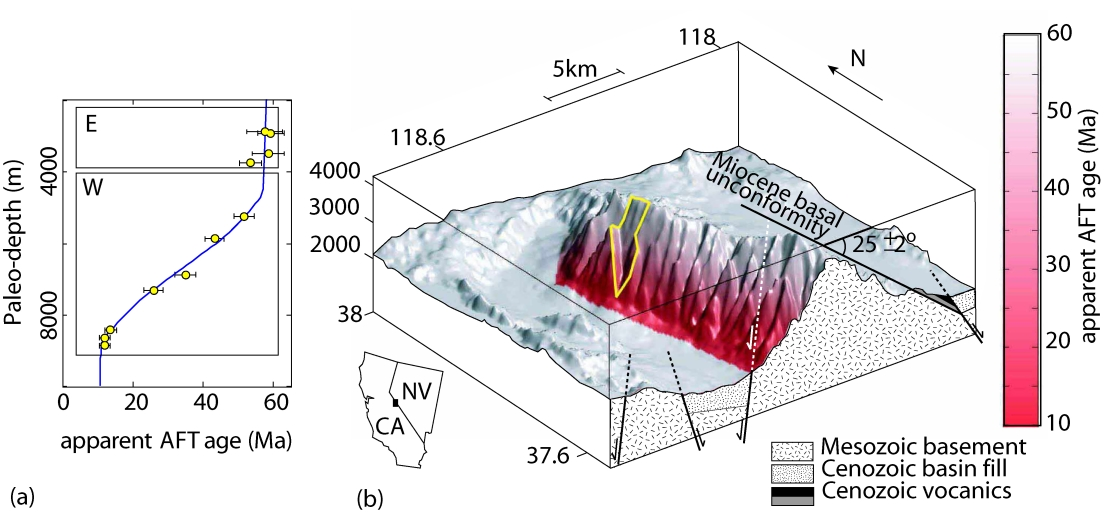
\includegraphics[width=\textwidth]{fig1.jpg}
  \caption[Predicted AFT cooling ages of the northern White Mountains]
  { (a) The AFT data of {\it Stockli et al.}  [2000] reveal an exhumed
    Partial  Annealing Zone  (PAZ).  Each  paleodepth under  a Miocene
    erosional unconformity corresponds to  a unique AFT age. The lower
    part of  this curve is  exposed on the  western side of  the range
    (box  labeled ``W''),  whereas the  upper part  is exposed  on the
    eastern side  (box labeled  ``E''). (b) For  each location  on the
    northern White Mountains, the paleodepth was calculated, and using
    (a), the corresponding AFT age was computed, and color-coded.  The
    yellow polygon outlines the Marble Creek drainage basin.}
\label{fig:whitePAZ}
\end{figure}

{\it Stockli et  al.}  [2000] measured AFT and  apatite (U-Th)/He ages
along   a  transect   in   the  northern   White  Mountains   (Figures
\ref{fig:whitePAZ}   and  \ref{fig:landsat}),  revealing   an  exhumed
fission     track    Partial     Annealing    Zone     (PAZ,    Figure
\ref{fig:whitePAZ}.a).   Defining ``paleodepth'' as  the perpendicular
distance  to the  assumed tilted  mid-Miocene erosional  surface, each
paleodepth in Figure \ref{fig:whitePAZ}.a  corresponds to a unique AFT
age and conversely,  each AFT age corresponds to  a unique paleodepth. 
AFT ages can  be predicted by computing the  paleodepth for each pixel
of a  digital elevation model  (DEM), and assigning  the corresponding
AFT age  to it.  This  is exactly how Figure  \ref{fig:whitePAZ}.b was
generated.  The paleodepth  values of {\it Stockli et  al.} [2000] are
based on  the interpretation that a  bedding dip in  the eastern White
Mountains  could be  reliably projected  across the  range  into space
(Figure  \ref{fig:whitePAZ}.b).  It  is, however,  possible  that this
surface was  folded, potentially causing  significant uncertainties on
the  paleodepths.   This  would  have  little  or  no  effect  on  the
reconstructed  AFT age-distribution.   Paleodepth is  just used  as an
intermediate step  between AFT age and topography.   Exactly via which
numerical  paleodepth-value an  AFT  age is  mapped  to a  topographic
location is irrelevant, as long as the mapping is correct.
\\

If  we assume that  the sand  grains were  uniformly derived  from the
entire drainage (assumption  2 of {\it Ruhl and  Hodges}, 2005), it is
possible to predict the detrital AFT grain-age distribution.  Detrital
thermochronological data are usually represented by estimates of their
probability density, whose interpretation often involves deconvolution
into Gaussian  subpopulations [{\it  Galbraith and Green},  1990; {\it
  Brandon},  1996].  Cumulative  distributions are  an  alternative to
probability density  estimates that have  recently gained considerable
popularity [{\it Brewer et al},  2003; {\it Amidon et al.}, 2005; {\it
  Ruhl  and Hodges},  2005; {\it  Hodges et  al.}, 2005].   This paper
introduces  a new kind  of cumulative  distribution which  is slightly
different from these previous studies.  The reasons why this so-called
``Cumulative  Age Distribution'' is  preferred to  probability density
estimates and previous cumulative  probability curves are discussed in
the following section.
\\

\begin{figure}[here]
  \centering
  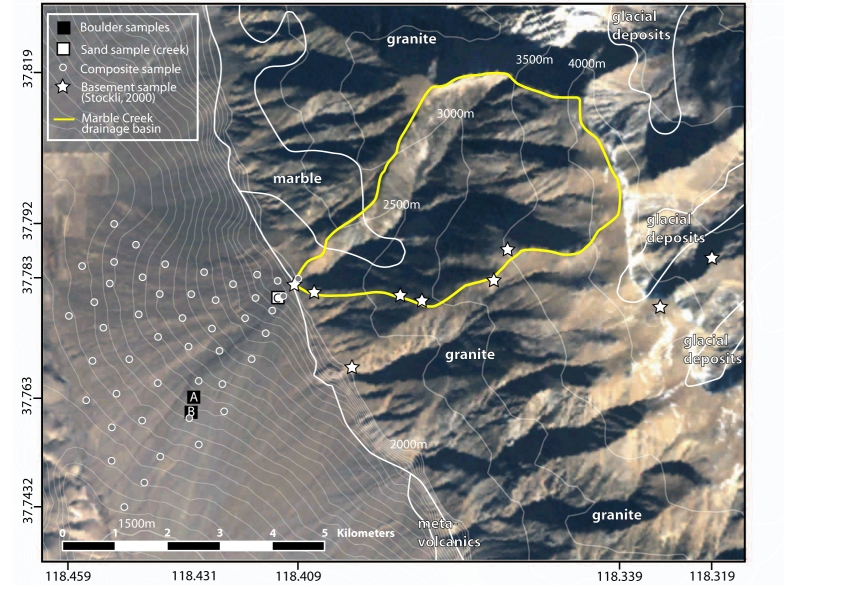
\includegraphics[width=\textwidth]{fig2.jpg}
  \caption[AFT sample locations]
  {Landsat image of  the Marble Creek drainage basin  and its alluvial
    fan, with  indication of the  sample locations and  the underlying
    geology, modified from {\it Saucedo  et al.} [2000] and {\it McKee
      and Conrad} [1996].}
\label{fig:landsat}
\end{figure}

\section{PDF vs. CSPDF vs. CAD}
\label{sec:pdfcspdfcad}

Detrital  thermochronological  age  distributions  can  be  visualized
either by  probability density estimates or  by cumulative probability
plots. For  the latter, two different kinds  of cumulative probability
diagrams  will  be  discussed.   The  various  acronyms  used  in  the
literature  are  summarized   in  Table  \ref{tab:definitions}.   This
section is an attempt to shed  a little light in this rather confusing
myriad of statistical tools.  Each  of the options will be defined and
compared with  its alternatives.  After  this section, only  the terms
``observed CAD'' and ``predicted CAD''  will be used.  Readers who are
just interested  in the  applications part of  this paper can  skip to
Section \ref{sec:application}.

\subsection{The Probability Density Function (PDF)}
The  information relevant  to  the kind  of detrital  thermochronology
discussed in  this paper  is not  so much the  actual ages,  but their
probability distribution.   Underlying any set  of detrital ages  is a
Probability  Density  Function (PDF),  describing  the probability  of
occurence of any detrital age t:

\begin{equation}
  \label{eq:pdf}
  Pr(a<t<b) = \int^b_a pdf(t) dt ~~~~~~~ \forall ~ a < b
\end{equation}

In practice, the PDF can  never be precisely known, because that would
require an exhaustive sampling of the detrital population.  Therefore,
we must work with {\it estimates}  of the PDF based on a finite sample
of  detrital  ages (typically  tens  to  hundreds  of ages).   Besides
limited data, measurement uncertainty  is a second factor reducing the
precision  of  density  estimates.   The most  popular  estimators  of
probability density are histograms and ``kernel density plots'' [e.g.,
{\it Silverman},  1986].  Both of  these methods apply some  degree of
``smoothing'' to the data, either by binning them into a histogram, or
by assigning a Gaussian uncertainty distribution to each measurement:

\begin{equation}
  \label{eq:pdfhat}
  \widehat{pdf}(t) = \frac{1}{n}\sum_{i=1}^{n}N (t|\mu = t_i, \sigma =
\alpha~\hat{\sigma}(t_i))
\end{equation}

With N(t$\mid\mu,\sigma$) the normal distribution of t with mean $\mu$
and standard  deviation $\sigma$, and  t$_i$ and $\hat{\sigma}$(t$_i$)
the measured  ages and their respective  1-$\sigma$ uncertainties.  To
illustrate  the different  approaches to  detrital thermochronological
density estimation, consider the degenerate case of a ``diving board''
hypsometry: all  detrital grains are derived from  a single elevation,
corresponding to a single ``true'' age t$_{true}$. The PDF of the true
ages  is  a  delta-function  (spike at  t$_{true}$,  zero  probability
elsewhere).   For further simplification,  all grains  have identical,
Gaussian  measurement uncertainties.  In  the following,  t$_{true}$ =
10Ma  so  all  grains  are  10Ma old  and  have  Gaussian  measurement
uncertainties of 1Ma.
\\

Suppose we have access to  an infinite number of measurement from this
detrital population.   The PDF of  these age measurements can  then be
determined  by a histogram  with infinitessimal  binwidth or  a kernel
density estimate  with infinitessimal $\alpha$.  Note that  the PDF of
the {\it  measurements} is not the  same as the PDF  of the underlying
{\it ages} (Figure  \ref{fig:divingBoardPdf}.a).  Unless we deconvolve
the  measurement  uncertainties,  the  measurement  distribution  will
always be a ``smoothed'' version of the ``true'' age distribution.  In
our toy example, the {\it  age distribution} is a delta-function at 10
Ma,  whereas   the  {\it  measurement  distribution}   is  a  Gaussian
distribution  with mean  10 Ma  and  standard deviation  1 Ma  (Figure
\ref{fig:divingBoardPdf}.a).
\\

\begin{figure}[htbp]
  \centering 
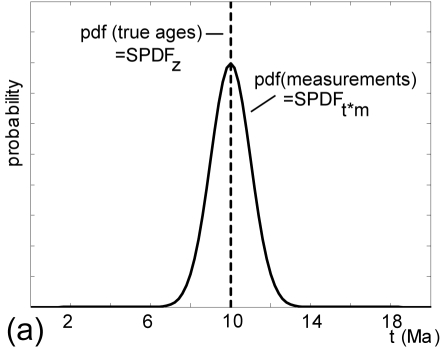
\includegraphics[width=.32\textwidth]{fig4a.jpg}
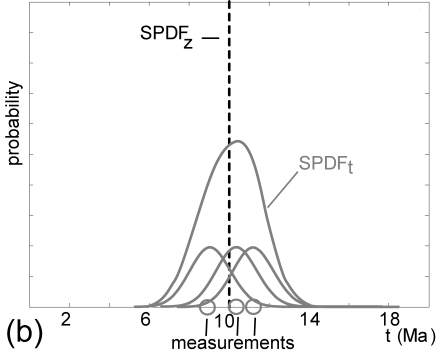
\includegraphics[width=.32\textwidth]{fig4b.jpg}
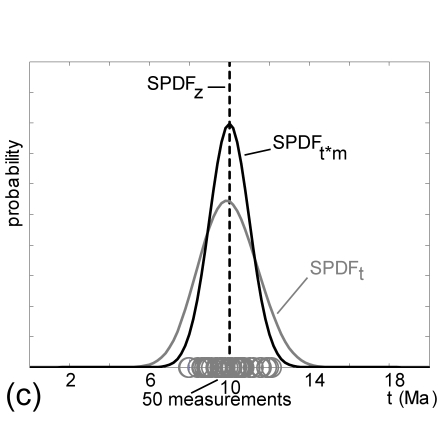
\includegraphics[width=.32\textwidth]{fig4c.jpg}
  \caption[Comparison of probability density estimators for a ``diving
  board  hypsometry'']  {(a)  dashed  line: expected  (errorless)  age
    distribution  of  a   ``diving  board''  hypsometry,  black  line:
    measurement  distribution  including  1Ma  (normally  distributed)
    measurement uncertainty; (b)  circles are three measurements drawn
    from the measurement distribution.  Using the nomenclature of {\it
      Ruhl and  Hodges} [2005], SPDF$_z$ is the  hypsometric curve and
    SPDF$_t$ is the Gaussian  kernel density estimator of the measured
    age distribution; (c) as  the number of measurements increases (50
    in this figure), SPDF$_t$  converges to a Normal distribution with
    standard deviation  $\sigma = \sqrt{2}$.   SPDF$_{t*m}$, which has
    been  used as  the  point of  comparison  between the  hypsometric
    predictions and  the measurements,  is a Normal  distribution with
    standard deviation $\sigma$ = 1.}
  \label{fig:divingBoardPdf}
\end{figure}

Given a set of age  data, the Gaussian kernel density estimator stacks
a bell curve on top  of each measurement (Equation \ref{eq:pdfhat} and
Figure \ref{fig:divingBoardPdf}.b).  Repeating this for a large number
of measurements  drawn from our  ``diving board'' hypsometry  yields a
Gaussian distribution with mean  10 Ma and standard deviation $\sigma$
= $\sqrt{(1  Ma)^2 + (\alpha \times 1  Ma)^2}$.  Thus, $\widehat{pdf}$
is ``double-smoothed'':  once by the measurement  uncertainties, and a
second time by the construction  of the kernel density estimator.  The
amount  of additional  smoothing depends  on the  parameter  $\alpha$. 
Although it  can be shown  that $\alpha$ =  0.6 is an optimal  value [
{\it Silverman}, 1986; {\it  Brandon}, 1996], previous studies by {\it
  Brewer et al.}  [2003], {\it  Ruhl and Hodges} [2005] and {\it Stock
  et  al.}   [2006]  have  used  $\alpha$  = 1,  and  so  does  Figure
\ref{fig:divingBoardPdf}.b.   {\it Ruhl and  Hodges} [2005]  gave this
curve  the  name ``Synoptic  Probability  Density  Function'' (SPDF).  
These authors distinguish between  three kinds of SPDF.  SPDF$_{z}$ is
the  true underlying  age distribution,  in the  hypothetical  case of
errorless      measurements      (dashed      lines     in      Figure
\ref{fig:divingBoardPdf}).  In  our toy  example, SPDF$_z$ is  a delta
function.   SPDF$_{t}$ is  the kernel  density estimator  generated by
Equation      \ref{eq:pdfhat}      (gray      lines     in      Figure
\ref{fig:divingBoardPdf}).   Finally, SPDF$_{t*m}$ effectively  is the
PDF     of    the    measurements     (black    lines     in    Figure
\ref{fig:divingBoardPdf}).   Because  SPDF$_{t*m}$  is  only  smoothed
once,  whereas SPDF$_{t}$  is  smoothed twice,  SPDF$_{t}$  is a  {\it
  biased} estimator of SPDF$_{t*m}$ (Figure
\ref{fig:divingBoardPdf}.c).\\

One of the requirements for the application of Gaussian kernel density
estimation  is   that  the  measurement   uncertainties  are  normally
distributed.     This   may   be    a   reasonable    assumption   for
$^{40}$Ar/$^{39}$Ar thermochronology, but  not necessarily for fission
tracks, which  are governed by  a Poisson process.  However,  by using
the logistic transform,  a set of fission track data  can be recast in
terms of a  new parameter z [{\it Brandon},  1996], which is estimated
by

\begin{equation}
  \label{eq:z}
  \hat{z} = ln(\lambda \zeta \ g \rho_D) + ln(\frac{N_s + 0.5}{N_i + 0.5})
\end{equation}

where    $\lambda$    is    the    decay   constant    of    $^{238}$U
(=1.55125$\times$10$^{-10}$a$^{-1}$),  $\zeta$  a  (zeta)  calibration
factor measured on  an AFT age standard, g  a geometric factor (=0.5),
N$_s$ the  number of spontaneous  fission tracks, N$_i$ the  number of
induced  tracks in  a mica  detector  and $\rho_D$  the induced  track
density of a glass standard that was irradiated along with the sample.
N$_s$  and N$_i$  are  Poisson variables,  but  $\hat{z}$ is  normally
distributed with standard error

\begin{equation}
  \label{eq:sez}
  \hat{\sigma}(z) = \sqrt{\frac{1}{N_s+0.5} + \frac{1}{N_i+0.5}}
\end{equation}

\subsection{The Cumulative Synoptic Probability Density Function (CSPDF)}

The  probability density function  (PDF) is  intimately linked  to the
cumulative density  function (CDF).  The  relationship between PDF
and CDF is:

\begin{eqnarray}
  \label{eq:pdfcdf}
  cdf(t) & = & \int_{-\infty}^t pdf(x) dx\\
  pdf(t) & = & \frac{d(cdf(t))}{dt}
\end{eqnarray}

PDF and  CDF are standard  statistical terms.  In the  nomenclature of
{\it Ruhl and  Hodges} [2005], the specific case  of a Gaussian kernel
density  estimator  with   $\alpha$  =  1  is  named   SPDF,  and  the
corresponding CDF is named the Cumulative Synoptic Probability Density
Function (CSPDF).  Thus, the CSPDF is defined by using SPDF instead of
PDF  in  Equation  \ref{eq:pdfcdf}.    Although  SPDF  and  CSPDF  are
interchangeable  from  a statistical  point  of  view,  the CSPDF  has
recently gained  considerable popularity for two  reasons.  First, the
cumulative  distribution  has  intuitive  significance, as  its  shape
mimics the  shape of the  the cumulative hypsometry (modulated  by the
age-elevation curve).   A second advantage of cumulative  plots is the
ease of  comparing different datasets by  using the Kolmogorov-Smirnov
(K-S) goodness-of-fit  test.  The K-S  test determines if  the maximum
vertical  distance   between  two  cumulative   distributions  can  be
explained by  random sampling effects  alone.  As illustrated  by {\it
  Amidon et al.}  [2005], using  the CSPDF in combination with the K-S
test is a useful tool for comparing two detrital datasets. However, we
will next see that the CSPDF  should {\it not} be used for the purpose
of comparing a detrital age distribution with hypsometric predictions.
\\

Revisiting the toy  example of a ``diving board''  hypsometry, the CDF
of  the true  ages is  a step-function  at t$_{true}$  =  10Ma (Figure
\ref{fig:cspdf50}).   The   theoretical  CDF  of   the  measured  ages
($\approx$ CSPDF$_{t*m}$ curve of {\it  Ruhl and Hodges}, 2005) is the
cumulative normal  distribution with mean 10Ma  and standard deviation
1Ma  (red  curve  on  Figure  \ref{fig:cspdf50}).   In  contrast,  the
cumulative kernel  density estimator  CSPDF$_t$ (gray curve  on Figure
\ref{fig:cspdf50})  is the  cumulative normal  distribution  with mean
10Ma  and standard deviation  $\sqrt{2}$Ma. Thus,  CSPDF$_t$ is  not a
good estimator of  CSPDF$_{t*m}$, for the same reason  why SPDF$_t$ is
not     a      good     estimator     of      SPDF$_{t*m}$     (Figure
\ref{fig:divingBoardPdf}).  In  other words, the  CSPDF is not  a good
tool  for comparing  detrital datasets  with  hypsometric predictions,
which  is exactly  the goal  of this  paper.  Fortunately,  the misfit
caused  by the  ``double  smoothing'' of  CSPDF$_t$  does not  greatly
affect the conclusions of {\it  Ruhl and Hodges} [2005] and {\it Stock
  et  al.}   [2006], because  the  analytical  uncertainties of  their
$^{40}$Ar/$^{39}$Ar  and  (U-Th)/He data  are  relatively small.   The
situation would be worse for the less precise AFT data presented here.
\\

\begin{figure}[][h]
\centering 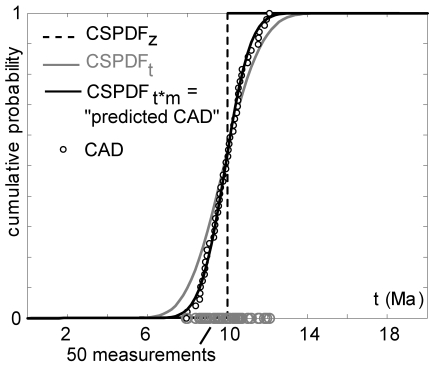
\includegraphics[width=.5\textwidth]{fig5.jpg}
\caption
[Cumulative density estimators for  the ``diving board hypsometry''] {
  The cumulative equivalent of Figure \ref{fig:divingBoardPdf}.c.  The
  dashed  step-function is  the  cumulative hypsometry  (CSPDF$_{z}$),
  corresponding to the ``true  age distribution'', which could only be
  measured if  we had access to errorless  measurements.  Gray circles
  are measurements, black circles  are the Cumulative Age Distribution
  (CAD).   The  black curve  is  CSPDF$_{t*m}$,  which coincides  with
  theoretical ``predicted  CAD'' obtained  from an infinite  number of
  synthetic  measurements  including  measurement uncertainties.   The
  observed CAD  is an  unbiased estimator of  the predicted  CAD.  The
  gray curve  is CSPDF$_{t}$ calculated  from the 50  measurements and
  their respective uncertainties.  CSPDF$_{t}$ is not a good estimator
  of CSPDF$_{t*m}$.  }
  \label{fig:cspdf50}
\end{figure}

The  CSPDF-method can be  ``fixed'' by  smoothing the  CSPDF$_{t*m}$ a
second  time.   In  practice,  CSPDF$_{t*m}$  can  be  constructed  by
collecting  a  large number  of  synthetic  ``measurements'' from  the
hypsometry  and adding  a synthetic  measurement error  to  them.  The
second smoothing step would then  involve stacking a bell curve on top
of each of the sythetic  measurements, as in Equation \ref{eq:pdfhat}. 
Instead of  this cumbersome  ``fix'', the Cumulative  Age Distribution
(CAD) is introduced as a simpler alternative to the CSPDF method.

\subsection{The Cumulative Age Distribution (CAD)} \label{sec:CAD}

One   of  the   most  significant   advantages  of   using  cumulative
distributions  instead   of  probability  density   estimates  is  not
exploited  by  the  CSPDF.   Whereas  it is  impossible  to  visualize
probability densities without using  at least some degree of smoothing
(either by binning  or by stacking Gaussian kernels),  this is not the
case  for cumulative distributions.   The Cumulative  Age Distribution
(CAD)  is  a  discrete  step-function  with the  sorted  detrital  age
measurements on  the x-axis and  their respective ranks on  the y-axis
(Figure \ref{fig:cspdf50}).  The (measured  or ``observed'') CAD is an
unbiased  estimator of  {\it  Ruhl and  Hodges}' [2005]  CPDF$_{t*m}$,
which will hereafter be named the ``predicted CAD''.
\\

At first glance,  it seems like the CAD does  not properly account for
variable measurement  uncertainties.  The CSPDF  explicitly takes into
account  analytical  uncertainties  ($\hat{\sigma}(t_i)$  in  Equation
\ref{eq:pdfhat}),  by ``spreading  out''  imprecise measurements  with
wider Gaussian kernels. In contrast  with this, the observed CAD gives
equal ``weight'' to all measurements. The observed CAD gets around the
need for kernel smoothing by shifting the uncertainty weighting to the
predicted CAD.  The  predicted CAD is computed from  the hypsometry by
simulating  the  detrital  sampling   process.   First,  a  number  of
synthetic  {\it  ages}  are  generated  from  the  hypsometry.   Then,
synthetic  measurement  errors are  added  to  each  of these  values,
comparable in  size to the real analytical  uncertainties.  From these
synthetic {\it measurements}, a predicted CAD is calculated in exactly
the same way as the observed CAD.  Thus, the measurement uncertainties
are properly accounted for by the  predicted CAD, and there is no need
to add  them to the  observed CAD a  second time.  Note that  the same
procedure is  also part of  the CSPDF-method, because  the ``predicted
CAD''  is  essentially the  same  as  {\it  Ruhl and  Hodges}'  [2005]
CSPDF$_{t*m}$.

\subsection{Taking into account unequal measurement uncertainties}
\label{sec:unequal}

In  the  toy example  discussed  before,  all  measurements had  equal
measurement  uncertainties. This  is  seldom the  case  in real  world
applications,  particularly when  fission  track dating  is involved.  
Most importantly,  AFT age uncertainties  are a sensitive  function of
the  number of spontaneous  fission tracks.   Young grains  have fewer
spontaneous tracks than older grains of similar U-concentration.  This
results in  widely variable  measurement uncertainties ranging  from a
few  percent for  old, U-rich  grains to  more than  100\%  for U-poor
grains containing  little or no  fission tracks.  As explained  in the
previous  section, measurement uncertainties  are incorporated  in the
predicted,  rather than  the  observed CAD.   The  problem of  unequal
measurement uncertainties  can be  mitigated by using  {\it Brandon}'s
[1996]   logarithmic  ``z-transformation''   (Equation   \ref{eq:z}).  
Although  this  is   a  valid  approach,  we  will   use  the  regular
age-equation in the following.
\\

The sand  and gravel samples discussed  in this paper  were dated with
the external detector method [{\it  Hurford and Green}, 1983]. The age
equation for this method is:

\begin{equation}
  \label{eq:EDTageEquation}
  t =  \frac{1}{\lambda}ln\left( 1+ \lambda \zeta  g \rho_D \frac{N_s}{N_i} \right)
\end{equation}

with  all variables  as in  Equation \ref{eq:z}.   Using  the external
detector method,  fission track ages  (t) are roughly  proportional to
the ratio of the expected  number of spontaneous tracks (N$_s$) in the
mineral  grain to  the expected  number of  tracks induced  by neutron
irradiation  (N$_i$):   t~$\propto$~N$_s$/N$_i$.   However,  if  N$_s$
and/or N$_i$ are small numbers  ($<$10), then the {\it observed} ratio
of  spontaneous  ($\hat{N}_s$)  to  induced ($\hat{N}_i$)  tracks  can
potentially be very different.  For example, if N$_s$=2, there is 14\%
chance    that    $\hat{N}_s$=0,    resulting    in   an    AFT    age
$\hat{t}\propto\hat{N}_s/\hat{N}_i$~=~0.   Assuming that  there  is no
systematic   correlation  between   N$_i$   and  t,   the  effect   of
Poisson-distributed counting  statistics on the CAD can  be modeled as
follows:

\begin{enumerate}
\item  Consider a probability  distribution of  AFT ages,  for example
  k = 1000 numbers drawn from the cumulative hypsometry.
\item For each of  these ages t$_j$ (1$\leq$j$\leq$k), randomly select
  a  N$_i$ value  ($N_i^j$,  say) from  the  database of  measurements
  (Tables 5 and 6 of the auxiliary material).
\item  Compute  the  expected   number  of  fission  tracks  ($N_s^j$)
  corresponding   to  t$_j$  and   N$_i^j$  by   rearranging  Equation
  \ref{eq:EDTageEquation}:

\begin{equation}
  \label{eq:modifiedAgeEquation}
N_s^j = \frac{N_i^j}{\lambda \zeta  g \rho_D} \left( e^{\lambda t_j} - 1 \right)
\end{equation}

\item Generate random replicates  $N_s^{j*}$ of $N_s^j$ and $N_i^{j*}$
of $N_i^j$ by sampling at random from a Poisson distribution:

\begin{equation}
  \label{eq:poisson}
  N_s^{j*} \sim Poiss(N_s^j)\mbox{, and }N_i^{j*} \sim Poiss(N_i^j)
\end{equation}

\item  Plug   $N_s^{j*}$,  $\zeta^j$  and   N$_i^{j*}$  into  Equation
  \ref{eq:EDTageEquation}.  This yields a replicate age t$_j^*$. Doing
  this for all k errorless AFT ages from the expected CAD yields a new
  CAD   (the  ``predicted   CAD'')   that  does   take  into   account
  Poisson-distributed measurement  uncertainties.  Note that  this CAD
  effectively follows the definition  of {\it Ruhl and Hodges}' [2005]
  CSPDF$_{t*m}$ curve.
\end{enumerate}

\section{CADs of the Marble Creek catchment}
\label{sec:application}

\subsection{Predicted CAD}
\label{sec:predictedCAD}

We now return  to the White Mountains.  To  illustrate the application
of detrital  thermochronology to quantitative  geomorphology, consider
granitoid    (quartz   monzonite)   boulders    A   and    B   (Figure
\ref{fig:boulders})  on the  alluvial fan  that is  fed by  the Marble
Creek  drainage.  Large  boulders  of several  meters  diameter are  a
characteristic  feature of  the alluvial  fans of  the  northern Owens
Valley (e.g., Figure  16 of {\it Beaty}, 1963).  They  can be found up
to several  kilometers from  the range front  and are evidence  of the
exceptional power of  the rare flash floods and  debris flows that are
responsible for  the bulk  of sediment transport  on the  Marble Creek
alluvial fan [{\it Beaty}, 1963].   The Marble Creek catchment area is
15.82 km$^2$, 14.01 km$^2$ of  which consist of quartz monzonite, with
only a  small portion of Paleozoic marble  (Figure \ref{fig:landsat}). 
Boulders A and B both have  an AFT age of 10$\pm$2 Ma, indicating that
they   were   derived   from   the   base   of   the   range   (Figure
\ref{fig:boulders}).   This method  is easily  extended to  samples of
many, rather than one clast.  Sand  sample C was collected at the apex
of the alluvial fan (Figure \ref{fig:landsat}).  If erosion is assumed
to be uniform across the entire Marble Canyon, then we can calculate a
predicted age distribution by  exhaustively sampling all the pixels of
the digital elevation model (Figure \ref{fig:whitePAZ}) and predicting
their respective expected AFT cooling ages.
\\

\begin{figure}[here]
  \centering
  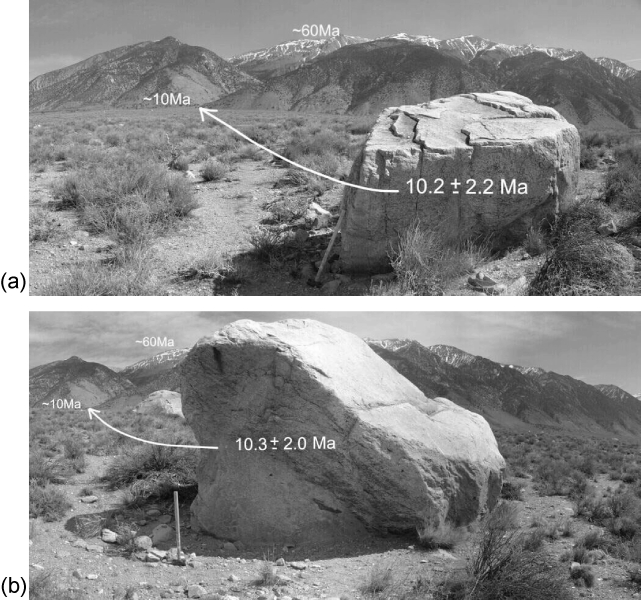
\includegraphics[width=.667\textwidth]{fig3.jpg}
  \caption[Boulders A and B]
  {Samples A  and B are large  granitic boulders on the  alluvial fan. 
    Their AFT age suggests that they were derived from the base of the
    mountain range. Sledge hammer ($\sim$80cm) for scale.}
\label{fig:boulders}
\end{figure}

Previous  studies [{\it Stock  and Montgomery},  1996; {\it  Brewer et
  al.}, 2003; {\it Ruhl and  Hodges}, 2005] assumed that exhumation is
laterally continuous and uniform.  In this case, the expected detrital
age  distribution   can  be   calculated  by  simply   convolving  the
age-elevation curve  with the  hypsometry.  In the  case of  the White
Mountains,  however,  it  is  known  that the  assumption  of  uniform
exhumation does not  hold, and that $\sim$ 25$^o$  of eastward tilting
has taken place  since the late Miocene [{\it Stockli  et al.}, 2003]. 
Therefore,  paleo-isotherms   are  not  horizontal,   and  the  simple
hypsometric approach is not valid.
\\

Relatively little  material will be derived from  the lower elevations
or higher paleodepths, because the basin is the narrowest at its mouth
(Figure \ref{fig:landsat}).  The CAD (Figure \ref{fig:obsCADs}) serves
as a  proxy for  the age-elevation curve  of the basement,  defined by
Figure  \ref{fig:whitePAZ}.a.  ``Steep''  parts  of the  age-elevation
curve are defined  by elevation intervals over which  the AFT ages are
approximately constant (Figure \ref{fig:whitePAZ}.a).  These ages will
be over-represented  in the  grain-age distribution and  correspond to
steep parts  of the  CAD.  Likewise, relatively  flat portions  of the
age-elevation curve correspond to intervals of the basement over which
the  AFT ages  change  rapidly  with elevation.   These  ages will  be
under-represented   in  the   detrital   grain-age  distribution   and
correspond  to  relatively  flat  parts  of  the  CAD.   Marble  Creek
sediments  only sample  ages corresponding  to the  lower part  of the
basement age-elevation curve.  Older ages can be found in sediments on
the eastern side of the mountain range (Figure \ref{fig:whitePAZ}).
\\

\begin{figure}[here]
  \centering
  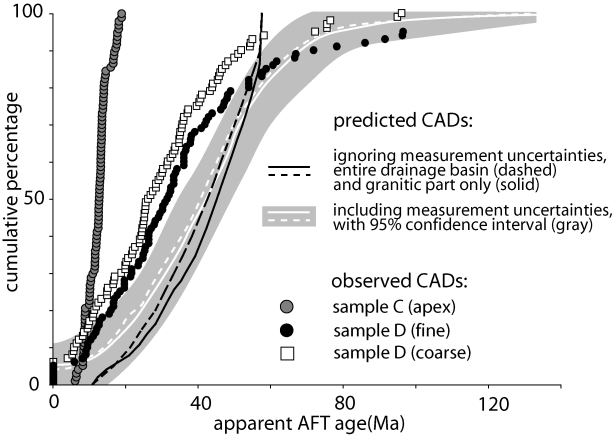
\includegraphics[width=.667\textwidth]{fig6.jpg}
  \caption[Observed CADs]
  {Comparison of predicted (line symbols) and observed (point symbols)
    CADs.  The  gray band contains 95\%  of all possible  CADs for the
    granitic  part  of the  catchment,  assuming  uniform erosion  and
    taking into account Poisson-based measurement uncertainties.}
\label{fig:obsCADs}
\end{figure}

The predicted  CAD shown in black on  Figure \ref{fig:obsCADs} assumes
zero  measurement uncertainties.  According  this curve,  the youngest
expected detrital  AFT grain-age should  be 12Ma, or 10Ma  taking into
account the measurement uncertainties reported by {\it Stockli et al.}
[2000].  However, the observed CAD  is not computed from composites of
many  apatites,  as  in  {\it  Stockli  et  al.}   [2000]  and  Figure
\ref{fig:whitePAZ}.a,  but on  individual AFT  grain-ages,  which have
much larger uncertainties that are governed by a Poisson distribution.
Using the database of  measured $\hat{t}$, $\hat{N}_s$ and $\hat{N}_i$
values provided  in the auxiliary  material, Section \ref{sec:unequal}
explained how to compute an equivalent predicted CAD that accounts for
these uncertainties (the white curve in Figure \ref{fig:obsCADs}).
\\

Apart from the measurement uncertainties inherent to the fission track
method,  additional uncertainty  is  introduced by  the finite  sample
size, 97-100 apatite  grains for this study. This  ensures us that the
largest population fraction that  was not missed with 95\% probability
is less  than 6\% of the  total [{\it Vermeesch},  2004].  5000 random
replicates of the predicted  CAD were generated by repeatedly sampling
97-100  times from  the  predicted age  distribution  (white curve  of
Figure  \ref{fig:obsCADs}),  and selecting  the  4750 replicates  that
yielded   the  smallest   Kolmogorov-Smirnov  (K-S)   statistic  [{\it
  Conover}, 1999] when compared to the predicted CAD (solid black line
in Figure  \ref{fig:obsCADs}).  Thus, the gray  confidence band around
the   predicted  CAD  of   Figure  \ref{fig:obsCADs}   represents  the
statistical uncertainty of the observed CADs. Please note that we just
use  the K-S  {\it statistic}  and not  the K-S  {\it test}.   The K-S
statistic is the largest vertical distance between two CDFs.  Based on
this statistic, {\it Kolmogorov} [1933] and {\it Smirnov} [1939, 1948]
devised  a test  to decide  whether or  not sampling  statistics alone
could  be responsible for  the difference  between two  distributions. 
This test  does not account  for the measurement uncertainties  of the
data.  However,  this is  irrelevant to the  extent that only  the K-S
statistic, and  not the  actual K-S test  is used for  calculating the
confidence band of Figure \ref{fig:obsCADs}.
\\

The studies  of {\it Brewer et  al.} [2004] and {\it  Ruhl and Hodges}
[2005] were located  in a very remote and  challenging Himalayan field
area, with  relatively poorly known lithology and  structural geology. 
Because these  conditions made  it very hard  to assess  the potential
impact  of non-uniform  lithology and  differential  exhumation, these
factors  were not  discussed in  much  detail. {\it  Ruhl and  Hodges}
[2005] list non-uniform lithology  and differential uplift under their
assumption  2.   They argue  that  if  the  observed CAD  matches  the
hysometry,  this can be  seen as  evidence for  the validity  of these
assumptions.   In  contrast with  these  previous  studies, the  White
Mountains  in general,  and the  Marble Creek  drainage  in particular
provide an excellent  testing ground for the CAD  method, because both
structure and  lithology are simple.   Nearly the entire  catchment is
underlain by a single pluton, the Pelissier Flats monzo-granite, which
is  bounded  to  the  West  by  a single  normal  fault,  but  remains
unaffected   by  faulting   elsewhere.    One  potentially   important
lithological inhomogeneity  are the mylonites of  the Cretaceous White
Mountain shear  zone [{\it Stockli  et al.}, 2003].  As  a first-order
test of  relatively uniform composition,  note that all  the Pelissier
Flats samples of  {\it Stockli et al.}  [2000,  2003] yielded abundant
apatite.   A small  but significant  part of  the canyon  is Paleozoic
marble  [{\it Crowder  et al.},  1972; Figure  \ref{fig:landsat}] that
contains no  apatite and will not  contribute to the  CAD.  The dashed
lines on  Figure \ref{fig:obsCADs} were calculated  assuming a uniform
lithology with uniform apatite  concentration.  The two solid lines on
Figure \ref{fig:obsCADs} show  the equivalent predicted CADs excluding
the marble  outcrop; their  difference illustrates the  sensitivity of
the  CAD  to lithological  inhomogeneity,  which  appears  to be  only
moderately important.

\subsection{Using the CAD for quantitative geomorphology by comparing observed
  with predicted CADs}
\label{sec:observedCAD}

The gray circles on Figure  \ref{fig:obsCADs} show the observed CAD of
sample  C (sand  collected  at the  apex  of the  alluvial fan).   The
difference with  the predicted CAD is immediately  apparent.  A useful
tool   for   comparing   two   (cumulative)   distributions   is   the
quantile-quantile (Q-Q) plot  [p.  353 of {\it Rice},  1995]. In a Q-Q
plot, the quantiles  of one distribution are plotted  against those of
another.  Two distributions are equal if  and only if they plot on the
1:1-line.  This is clearly not the  case for the CAD of sample C (gray
circles on  Figure \ref{fig:QQplot}). Sample C consists  of very young
ages between 6  and 19Ma indicating that it was  derived from very low
elevations.  This very localized  provenance of sample C suggests that
sediments  in the  presently active  Marble Creek  are derived  from a
single rock fall event localized very close to the mouth of the Marble
Creek  drainage, at  an elevation  of at  most 500m  above  the sample
location (Figures \ref{fig:whitePAZ} and \ref{fig:landsat}).
\\

\begin{figure}[here]
  \centering
  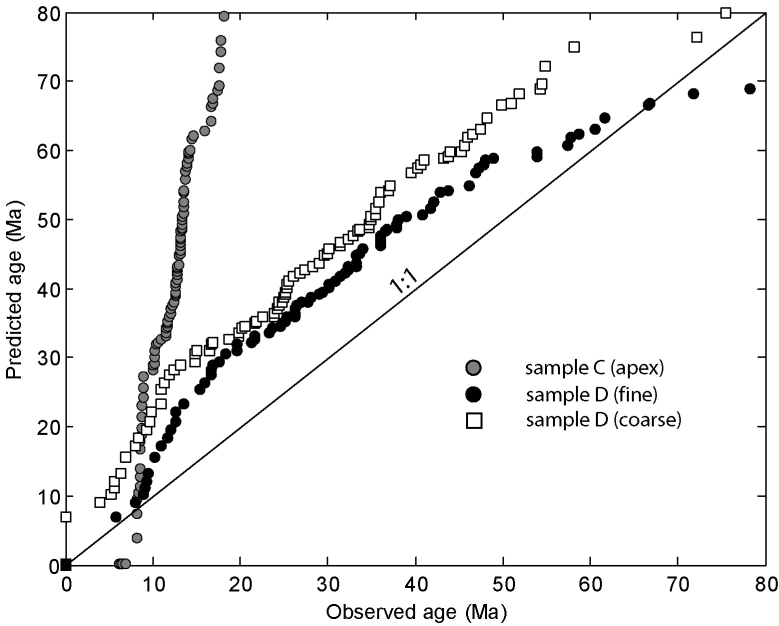
\includegraphics[width=.667\textwidth]{fig7.jpg}
  \caption[Q-Q plot]
  {Quantile-quantile (Q-Q) plot of  expected versus observed AFT ages. 
    Young  ages are  overrepresented  in sample  C  (single sample  of
    sand),  indicating that it  was derived  from low  elevations. The
    CADs  of  the composite  sample  D  are  closer to  the  predicted
    distribution,  indicating that  over longer  timescales, sediments
    are  derived  from  the   entire  drainage,  albeit  with  greater
    contributions from lower elevations than from further away.}
\label{fig:QQplot}
\end{figure}

Thus far, we have  studied clasts A and B and a  single sand sample C. 
The next logical  study is a composite of the  entire alluvial fan, in
an attempt to get a more integrated view of the entire drainage basin.
47 samples  were collected from all  over the alluvial  fan (sample D:
circles on  Figure \ref{fig:landsat}).   These samples can  be jointly
considered, because  the time span  covered by fan surfaces  in debris
flow dominated alluvial  fans of the Owens Valley  is relatively short
($<$  100ka;  {\it D\"{u}hnforth  et  al.},  2007).   To estimate  the
possible  importance of  grain-size induced  bias, these  samples were
divided into a coarse (5 cm $>$ clasts $>$ 7.925 mm) and a fine (2.794
mm $>$ clasts $>$ 0.595 mm)  fraction.  Then, the samples from each of
the  two  groups  were mixed  and  dated  with  the AFT  method.   The
resulting CADs are shown as  white squares and black circles on Figure
\ref{fig:obsCADs}.  Most  apatites in  the composite sample  are older
than sample  C.  The  coarse fraction appears  to be  slightly younger
than  the  fine fraction,  but  the  difference  is not  statistically
significant (compare the distance between  the two CADs with the width
of the gray  confidence band in Figure \ref{fig:obsCADs}),  and we may
conclude that grain-size  effects are not very important.   Just as we
did  for sample  C, we  compare the  observed and  predicted  CADs for
sample D  by plotting  them on a  Q-Q plot (Figure  \ref{fig:QQplot}). 
This analysis indicates that the composite sample was derived from the
entire  drainage.    Most  of  the  sediment  was   derived  from  low
elevations, with smaller contributions from further away.
\\

$\sim$ 5\%  of the  detrital grains in  sample D  have a zero  AFT age
whereas other apatites  appear to be well over  100 Ma old, apparently
contradicting the  10-55 Ma  age range predicted  by the  PAZ-curve of
{\it Stockli et al.}  [2000].  At first glance, this observation seems
to  suggest that  some apatites  are derived  from outside  the Marble
Creek catchment.   There are  at least two  possible sources  for such
``contamination'': (1) the catchment is down wind from the Long Valley
caldera, and  the area was likely  covered by a thick  layer of Bishop
volcanic ash; and (2) eolian  processes in the arid Owens Valley might
contaminate the Marble Creek alluvial fan with modern dust.  The first
possibility can be ruled  out because the relatively coarse grain-size
of  sample   D  allowed  verification   of  its  granite   and  marble
composition. Virtually  no tuff was  found.  The coarse  grain-size of
sample  D also drastically  reduces the  probability of  modern eolian
contamination.  Alternatively, the ``anomalous''  AFT ages can be much
more easily explained by  the counting statistics discussed in Section
\ref{sec:pdfcspdfcad}.
\\

\subsection{Suggestions for future improvements}
\label{sec:future}

The  CAD method would  gain considerable  power if  the AFT  data were
complemented by  (U-Th)/He measurements as  was done by {\it  Stock et
  al.}  [2007] for  two catchments in the Sierra  Nevada.  Whereas the
AFT CAD serves  as a proxy for the PAZ curve,  the (U-Th)/He CAD would
be  a proxy  for  the  Partial Retention  Zone  (PRZ) curve.   Because
(U-Th)/He  ages from the  northern White  Mountains have  already been
measured [{\it Stockli  et al.}, 2000], this would  be relatively easy
to   do.   Measurement  uncertainities   of  single   grain  (U-Th)/He
measurements  are approximately  normally  distributed, and  typically
much  smaller  than  single   grain  AFT  measurement  uncertainties.  
Unfortunately,  this is  only true  for inclusion-free  apatites.  The
vast majority  of igneous apatites  contain abundant $\alpha$-emitting
mineral  inclusions such  as zircon  and monazite,  and  the Pelissier
Flats  apatites  are  no  exception  to this.   In  basement  studies,
inclusion-free  apatites  are  carefully  selected under  a  binocular
microscope.  Not  only would doing this for  $\sim$100 detrital grains
be very  time consuming, it  would create potentially biased  samples. 
Therefore,   detrital   (U-Th)/He   studies   should   also   consider
inclusion-bearing grains [{\it Vermeesch et al.}, 2007].
\\

Another approach  to obtain more  and better information from  the AFT
data  is by  artificially increasing  the number  of  confined fission
tracks through heavy-ion irradiation  or exposure to $^{252}$Cf [e.g.,
{\it Ohira et  al.}, 1994].  Like the AFT  ages, fission track lengths
show a dependence on paleodepth (and thus elevation).  At low and high
paleodepths  well above  or below  the paleo-PAZ,  fission  tracks are
long, whereas  in the PAZ, short  tracks also exist.  Each  AFT age on
Figure   \ref{fig:whitePAZ}.a    corresponds   to   a   characteristic
distribution of  horizontally confined  fission track (HCFT)  lengths. 
Heavy ion  irradiation or bombardment by  $^{252}$Cf fission fragments
provides pathways through which the etching acid can reach more HCFTs,
up to  a point where  there is more  than one HCFT per  apatite grain,
even for samples with low  numbers of spontaneous fission tracks [{\it
  Ohira et al.}, 1994].  If the  HCFT lengths and AFT ages of the same
grains  are measured,  the provenance  paleodepth distribution  can be
determined more reliably  than by only using the  AFT ages. The Marble
Creek  catchment would be  the perfect  test-case for  this technique,
because the  HCFT-length distribution of  the basement is  known [{\it
  Stockli et al.}, 2000, 2003].

\section{Conclusions}

Apparent ages of low temperature thermochronometers generally decrease
with depth  below the surface.   When basement terranes  are uplifted,
this  variation produces an  age-elevation dependence.   Therefore, it
may be possible  to recover the provenance elevation  of the erosional
products of exhumed fault-blocks. This paper introduced the Cumulative
Age  Distribution  as  a  tool  for comparing  observed  detrital  age
distributions with hypsometric predictions.  The CAD is the cumulative
density  function of the  measured ages.  Arguably the  most important
advantage of the CAD over alternative approaches is that it visualizes
the  detrital sample without  the need  for data  smoothing. (Unequal)
measurement  uncertainties  are   incorporated  in  a  hypsometrically
predicted  CAD by  numerically simulating  the sampling  process.  The
statistical  variability caused  by  the combined  effects of  limited
sample size and analytical uncertainty can be estimated and visualized
with a bootstrapped confidence interval of the predicted CAD.\\

If  (1) apatite concentration  is uniform  across the  entire drainage
basin,  (2) measurement uncertainties  are small,  and (3)  erosion is
uniform  across  the entire  drainage  basin,  then a  hypsometrically
weighted CAD of detrital AFT data  has the same shape as the PAZ curve
of the  basement.  Under the  aforementioned assumptions, it  would be
possible to use the CAD  as a tool for paleo-relief reconstruction, by
studying sequential CADs through time, where the modern CAD is used to
calibrate  the older  ones  (i.e., convert  cumulative percentages  to
meters),  thus  taking  the  approach  suggested  by  {\it  Stock  and
  Montgomery} [1996] one step further.  Unfortunately, very few if any
field areas fulfill all three  requirements.  If assumption (3) is not
valid,  the method  is still  useful, because  testing  assumption (3)
yields useful  quantitative geomophological information.   The CADs of
the  White Mountains  reveal that  sediments in  the  currently active
Marble Creek  are derived  from a single  point source,  but composite
samples  of  the  entire  alluvial  fan are  derived  from  the  whole
catchment, with the  largest contributions from the base  of the range
and lower contributions from higher up the drainage.
\\

\begin{table}[here]
  \centering
\begin{footnotesize}
  \begin{tabular}[]{|p{.1\textwidth}|p{.8\textwidth}|}
\hline
term & definition \\
\hline\hline
PDF & Probability Density Function\\
\hline
CDF & Cumulative Density Function\\
\hline
SPDF,  CSPDF &  Synoptic   Probability  Density   Function  and
  Cumulative Synoptic Probability Density Function, respectively\\
\hline
SPDF$_{z}$ &  Hypsometry, i.e. the  probability (or area)  of any
  given elevation within a catchment\\
\hline
SPDF$_{t}$ & This curve is obtained from n age measurements by:
(1) assigning a Gaussian distribution to each age measurement with
    standard deviation equal to the measurement uncertainty,
(2) ``stacking'' all these Gaussian distributions, and
(3) normalizing the area under the resulting curve\\
\hline
CSPDF$_{z}$, CSPDF$_{t}$ &  Cumulative versions of SPDF$_{z}$ and
  SPDF$_{t}$, respectively\\
\hline
SPDF$_{z^*}$, SPDF$_{t^*}$,  CSPDF$_{z^*}$ and CSPDF$_{t^*}$ & In
  the nomenclature of {\it Ruhl and  Hodges} [2005], z$^*$ and t$^*$ are the
  normalized  versions  of  z  and  t,  respectively;  i.e.   z$^*$  =
  z/(max(z)-min(z))  and  t$^*$ =  t/(max(t)-min(t)).   Thanks to  the
  normalization,  elevations and  ages can  be directly  compared with
  each other.  In this paper, the  asterisks are
  dropped and it is clear from the context whether the normalized
  or the raw variables are used\\
\hline
CSPDF$_{t^*m}$ & A  ``model CSPDF$_t$-curve''.  If n measurements
  were used  to calculate SPDF$_t$,  then CSPDF${_t}$ is  calculated by
randomly selecting n points  from SPDF$_z$.  First, a nominal normally
distributed ``analytical  uncertainty'' like that of  the actual grain
ages  is  associated with  each  of  the  n elevations,  the  Gaussian
distributions  are summed, and  the resulting  curve is  normalized to
form a CSPDF$_{t^*m}$ curve\\
\hline
(Observed) CAD & ``Cumulative  Age Distribution'',
a discrete step-function with the sorted detrital age measurements 
on the x-axis and their respective ranks on the y-axis
\\
\hline
Predicted CAD &  Is  calculated by  randomly  selecting a  large
  number (e.g.  k  = 1000) of points from  SPDF$_{z}$, and assigning a
  synthetic ``measurement error''  to each of them by  adding a random
  number  from the  error distribution  of  one of  the n  measurement
  uncertainties of  the ``real'' measurements which were  used for the
  construction  of  SPDF$_{t}$  and  CSPDF$_{t}$.  The  k  ``synthetic
  measurements'' are  then sorted and plotted  as a CAD,  i.e.  
a discrete step-function with the sorted measurements 
on the x-axis and their respective ranks on the y-axis.  
Thus, the predicted CAD is practically identical to the CSPDF$_{t^*m}$\\
\hline\hline
  \end{tabular}
\end{footnotesize}
  \caption{Definition of acronyms used in the literature and in this paper}
  \label{tab:definitions}
\end{table}

\section*{Acknowledgments}

This work  was carried out  while the author  was a Ph.D.   student at
Stanford  University.   Many  thanks  to Mike  McWilliams  for  useful
comments on the first drafts of  the paper, and to Kate Huntington and
Kip Hodges  for statistical discussions.  This  paper greatly improved
over the  course of  three rounds of  review by Douglas  Burbank, Mark
Brandon, Daniel  Stockli, Kelin Whipple  and two anonymous  reviewers. 
Samples A, B and C were dated by Paul O'Sullivan of A2Z Inc.  Sample D
was dated by Geotrack International Pty.

\section*{References}

\begin{description}
  
\item Amidon,  W.H., D.W. Burbank,  and G.E. Gehrels (2005),  Construction of
  detrital mineral  populations, insights  from mixing of  U-Pb zircon
  ages in Himalayan rivers, {\it Basin Research, 17}, 463-485.
  
\item Beaty,  C.B. (1963), Origin  of alluvial fans,  White Mountains,
  California and  Nevada, {\it Annals  of the Association  of American
    Geographers, 53}, 516-535.

\item Brandon, M. T. (1996), Probability density plot for fission-track
grain-age samples, {\it Rad. Meas., 26}, 5, 663-676.

\item Brewer, I.D., Burbank,  D.W., and Hodges, K.V. (2003), Modelling
  detrital  cooling-age  populations:   insights  from  two  Himalayan
  catchments, {\it Basin Research, 15}, 305-320.
  
\item   Conover,   W.  J.    (1999),   {\it  Practical   nonparametric
    statistics}, 584 pp., John Wiley, New York.
  
\item Crowder,  D.  F., Robinson, P.   F., and Harris,  D. L.  (1972),
  {\it Geologic map of  the Benton Quadrangle, Mono County, California
    and Esmeralda and mineral counties, Nevada}, USGS, scale 1:62,500.
  
\item D\"{u}hnforth,  M., Densmore,  A.L., Ivy-Ochs, S.,  Allen, P.A.,
  Kubik,  P.W.   (2007),  Timing  and  patterns   of  debris-flow  fan
  deposition  on  Shepherd  and   Symmes  Creek  fans,  Owens  Valley,
  California, deduced from cosmogenic  $^{10}$Be. {\it Jour.  Geophys. 
    Res. Earth Surface} (in press).
  
\item Galbraith,  R.  F.,  and Green, P.   F.  (1990),  Estimating the
  component ages in  a finite mixture, {\it Nucl.   Tracks Rad. Meas.,
    17}, 3, 197-206.
  
\item Hodges, K.V.,  K.W. Ruhl, C.W. Wobus, and  M.S.  Pringle (2005),
  $^{40}$Ar/$^{39}$Ar Thermochronology  of Detrital Minerals,  in {\it
    Low temperature thermochronology: techniques, interpretations, and
    applications},  edited by  P.W.  Reiners,  and T.A.   Ehlers, {\it
    Rev. Mineral. Geochem., 58}, 239-257.
  
\item Hurford, A.J., and Green,  P.F. (1983), The zeta age calibration
  of fission track dating, {\it Isotope Geosc., 1}, 285-317.
  
\item  Kolmogorov, A.  (1933),  Sulla determinazione  empirica di  una
  legge di distributione, {\it Giornale dell' instituto Italiano degle
    attuari, 4}, 1-11.
  
\item McKee, E.  H., and Conrad, J. E.  (1996), A  tale of 10 plutons,
  revisited; age of granitic  rocks in the White Mountains, California
  and Nevada,  {\it Geol. Soc. Am.  Bull., 108}, 12,
  1515-1527.
  
\item Ohira, H., Heiguchi, K., Yoshimura, T., Komatsubara, T., Furuno,
  K., Kudo, H., and Hashimoto, T. (1994), Comparison of two methods of
  enhancing detection of confined fission tracks in minerals -- Ni ion
  irradiation  using   a  tandem  accelerator   and  fission  fragment
  irradiation using $^{252}$Cf source, {\it J. Geol. Soc. Japan, 100},
  2, 129-135.
  
\item Reheis, M.C., and T.H.   Dixon (1996), Kinematics of the eastern
  California  shear zone: Evidence  for slip  transfer from  Owens and
  Saline  Valley fault  zones to  Fish  Lake Valley  fault zone,  {\it
    Geology, 24}, 339-342.
  
\item Reheis, M.C., and T.L.  Sawyer (1997), Late Cenozoic history and
  slip rates of the Fish  Lake Valley, Emigrant Peak, and Deep Springs
  fault zones, Nevada and California, {\it Geol. Soc. Am. Bull., 109},
  280-299.
  
\item  Rice,  J.A.   (1995),  {\it Mathematical  statistics  and  data
    analysis}, 602 pp., Duxbury Press, Belmont, CA.
  
\item Ruhl, K.W., and Hodges, K.V. (2005), The use of detrital mineral
  cooling ages to evaluate steady state assumptions in active orogens:
  An example from the  central Nepalese Himalaya, {\it Tectonics, 24},
  doi:10.1029/2004TC001712
  
\item Saucedo, G.  J., Bedford, D.  R., Raines, G.  L., Miller, R. J.,
  and Wentworth, C.  M.  (2000), {\it GIS data for the geologic map of
    California}, compilated by Jennings, C.W.  (1977), {\it Cal.  Div.
    Mines Geol.}.
  
\item Silverman, B. W.  (1986), {\it Density estimation for statistics
    and  data analysis}, 175  pp., {\it  Monographs on  statistics and
    applied probability}, Chapman and Hall, London, New York.
  
\item  Smirnov,  H.  (1939),  Sur  les  \'{e}carts  de  la  courbe  de
  distribution     empirique,     {\it    Receuil     math\'{e}matique
    (Metematiceskii sbornik), 6}, 3-26.
  
\item Smirnov, H. (1948), Table for estimating the goodness of fit for
  empirical distributions, {\it Ann.  Math.  Stat., 19}, 279-281.
  
\item  Stewart, J.  H., (1988),  Tectonics  of the  Walker Lane  Belt,
  western Great Basin: Mesozoic and  Cenozoic deformation in a zone of
  shear,  in {\it Rubey  Volume, vol.   7}, edited  by Ernst,  W.  G.,
  Englewood Cliffs, Prentice-Hall, 683-713.
  
\item   Stock,   J.D.,  and   Montgomery,   D.R.  (1996),   Estimating
  palaeorelief from detrital mineral  age ranges, {\it Basin Research,
    8}, 317-327.
  
\item Stock,  G.M., T.A.  Ehlers, and K.A.  Farley (2006),  Where does
  sediment  come from?   Quantifying catchment  erosion  with detrital
  apatite (U-Th)/He thermochronometry, {\it Geology, 34}, 725-728.
  
\item Stockli,  D.  F.,  Farley, K.  A.,  and Dumitru, T.  A.  (2000),
  Calibration of the apatite (U-Th)/He thermochronometer on an exhumed
  fault  block, White  Mountains, California,  {\it Geology,  28}, 11,
  983-986.
  
\item Stockli, D.  F., Dumitru,  T. A., McWilliams, M. O., and Farley,
  K.  A.  (2003), Cenozoic  tectonic evolution of the White Mountains,
  California and Nevada, {\it Geol. Soc. Am. Bull., 115}, 7, 788-816.
  
\item  Vermeesch,  P.   (2004),  How  many grains  are  needed  for  a
  provenance  study?   {\it  Earth  Planet.  Sci.  Lett.,  224},  3-4,
  441-451.
  
\item  Vermeesch,  P.,  D.   Seward,   C.   Latkoczy,  M.   Wipf,  D.  
  G\"{u}nther,   and  H.    Baur  (2007),   $\alpha$-emitting  mineral
  inclusions in  apatite, their effect  on (U-Th)/He ages, and  how to
  reduce it, Geochim. Cosmochim. Acta, (in press).

\end{description}

\end{document}